 \chapter{ЭКОНОМИЧЕСКИЙ РАЗДЕЛ}
 \setcounter{page}{32}
\newpage

 \section{Введение в экономический раздел}

Целью дипломной работы является доработка системы дистанционного обучения МАИ с целью адаптации системы на основе поступающей инфор\-мации о времени, которое студент затрачивает для ответов на задачи в про\-цессе тестирования. На основании анализа времени ответа делается вывод о том, не было ли у студента заранее приготовленных ответов не задачи теста.

В основной части диплома описывается математическое обеспечение сис\-темы и программная реализация, которые в совокупности представляют со\-бой завершенный программный продукт, готовый для продажи на рынке программного обеспечения.

В экономической части диплома производится расчёт затрат, которые несёт заказчик программного обеспечения системы дистанционного обучения МАИ. Исходя из затрат формируется стоимость проекта. По результатам оценки стоимости проекта производится расчёт экономической эффективно\-сти. Так же на основании сетевого графика производится расчёт временных па\-раметров проекта и вероятность его успешного выполнения в установлен\-ный срок.

\section{Сетевой график}

Сетевой график представляет собой графическое отображение этапов ра\-бот, которые необходимо провести для завершения дипломного проекта. С помощью сетевого графика можно спрогнозировать общее время, которое потребуется для выполнения проекта, а так же вычислить вероятность вы\-полнения проекта в срок.

\subsection{Таблица этапов работ}
По каждому этапу дипломной работы указано минимальное время выпол\-нения этапа и максимальное время выпол\-нения этапа. Исходя из этих зна\-чений рассчитывается ожидаемое время, которое потребуется затратить на данный этап:
$$
t_{exp} = \frac{2t_{min}+3t_{max}}{5}
$$

Дисперсия времени работы вычисляется по формуле
$$
t_{exp} = \left( \frac{t_{max} - t_{min}}{5} \right)^2
$$

По результатам расчётов построим таблицу
%\begin{myTable}
\begin{center}
Таблица 2.2: Таблица этапов работ
\end{center}
{
\scriptsize
\begin{longtable}[H]{|p{0.9cm}|p{3.4cm}|p{1.4cm}|p{3.9cm}|p{0.6cm}|p{0.7cm}|p{0.6cm}|p{0.7cm}|}
%\caption{\normalsize Таблица этапов работ}}\\
\hline
Этап & Событие             & Шифр & Работа                                        & $t_{min}$ & $t_{max}$ & $t_{exp}$ & $\sigma$\\
\hline
1    & Изучение литературы & 1-4  & Изучение литературы по основной части диплома & 2         & 5         &  3,8      &  0,36    \\
\cline{3-8}
& &1-12&Изучение литературы по экономической части&3&6&4,8&0,36\\
\cline{3-8}&&1-10&Изучение литературы по охране труда и окружающей среды&1&4&2,8&0,36\\
\hline
2&Окончание доработки СДО&2-7&Анализ структуры и программного кода СДО&6&9&7,8&0,36\\
\hline
3&Получен список необходимых доработок&3-2&Доработка СДО для получения экспериментальных данных и оценки параметров модели&4&8&6,4&0,64\\
\hline
4&Необходимость построения математической модели&4-5&Изучение математических методов моделирования времени ответа в СДО&2&5&3,8&0,36\\
\hline
5&Завершение математической модели&5-6&Применение математической модели для анализа времени ответа&7&11&9,4&0,64\\
\cline{3-8}
&&5-2&Описание математической модели&6&9&7,8&0,36\\
\hline
7&Оценка параметров модели&7-8&Оценка по экспериментальным данным параметров модели &7&10&8,8&0,36\\
\cline{3-8}
&&7-9&Применение модели к реальным входным данным&2&5&3,8&0,36\\
\hline
8&Прогнозирование ответа на основании модели&8-9&Получение результатов обработки реальных данных&3&6&4,8&0,36\\
\hline
9&Построение таблиц, диаграмм, анализ полученных данных&9-14&Оформление результатов практической части&4&7&5,8&0,36\\
\hline
10&Раздел <<Охрана труда и окружающей среды>>&10-11&Написание теоретического материала раздела <<Охрана труда и окружающей среды>>&3&5&4,2&0,16\\
\hline
11&Расчет кондиционирования&11-14&Проведение расчётов&6&8&7,2&0,16\\
\hline
12&Раздел <<Экономическая эффективность>>&12-13&Написание теоретического материала раздела <<Экономическая эффективность>>&2&5&3,8&0,36\\
\hline
13&Построение сетевого графика&13-14&Проведение расчётов&6&9&7,8&0,36\\
\hline
14&Оформление готового диплома&-&Оформление полученных результатов&&&&\\
\hline
\end{longtable}
}
%\end{myTable}

\newpage

\subsection{Построение сетевой модели}

Построим на основании таблицы из п. (1.2.1) «Таблица этапов работ» сетевой график. Круги обозначают события, стрелками обозначены работы. Подписи над стрелками указывают ожидаемое время выполнения работы.
\\
\begin{figure}[ht!]
\label{setgr}
\centering 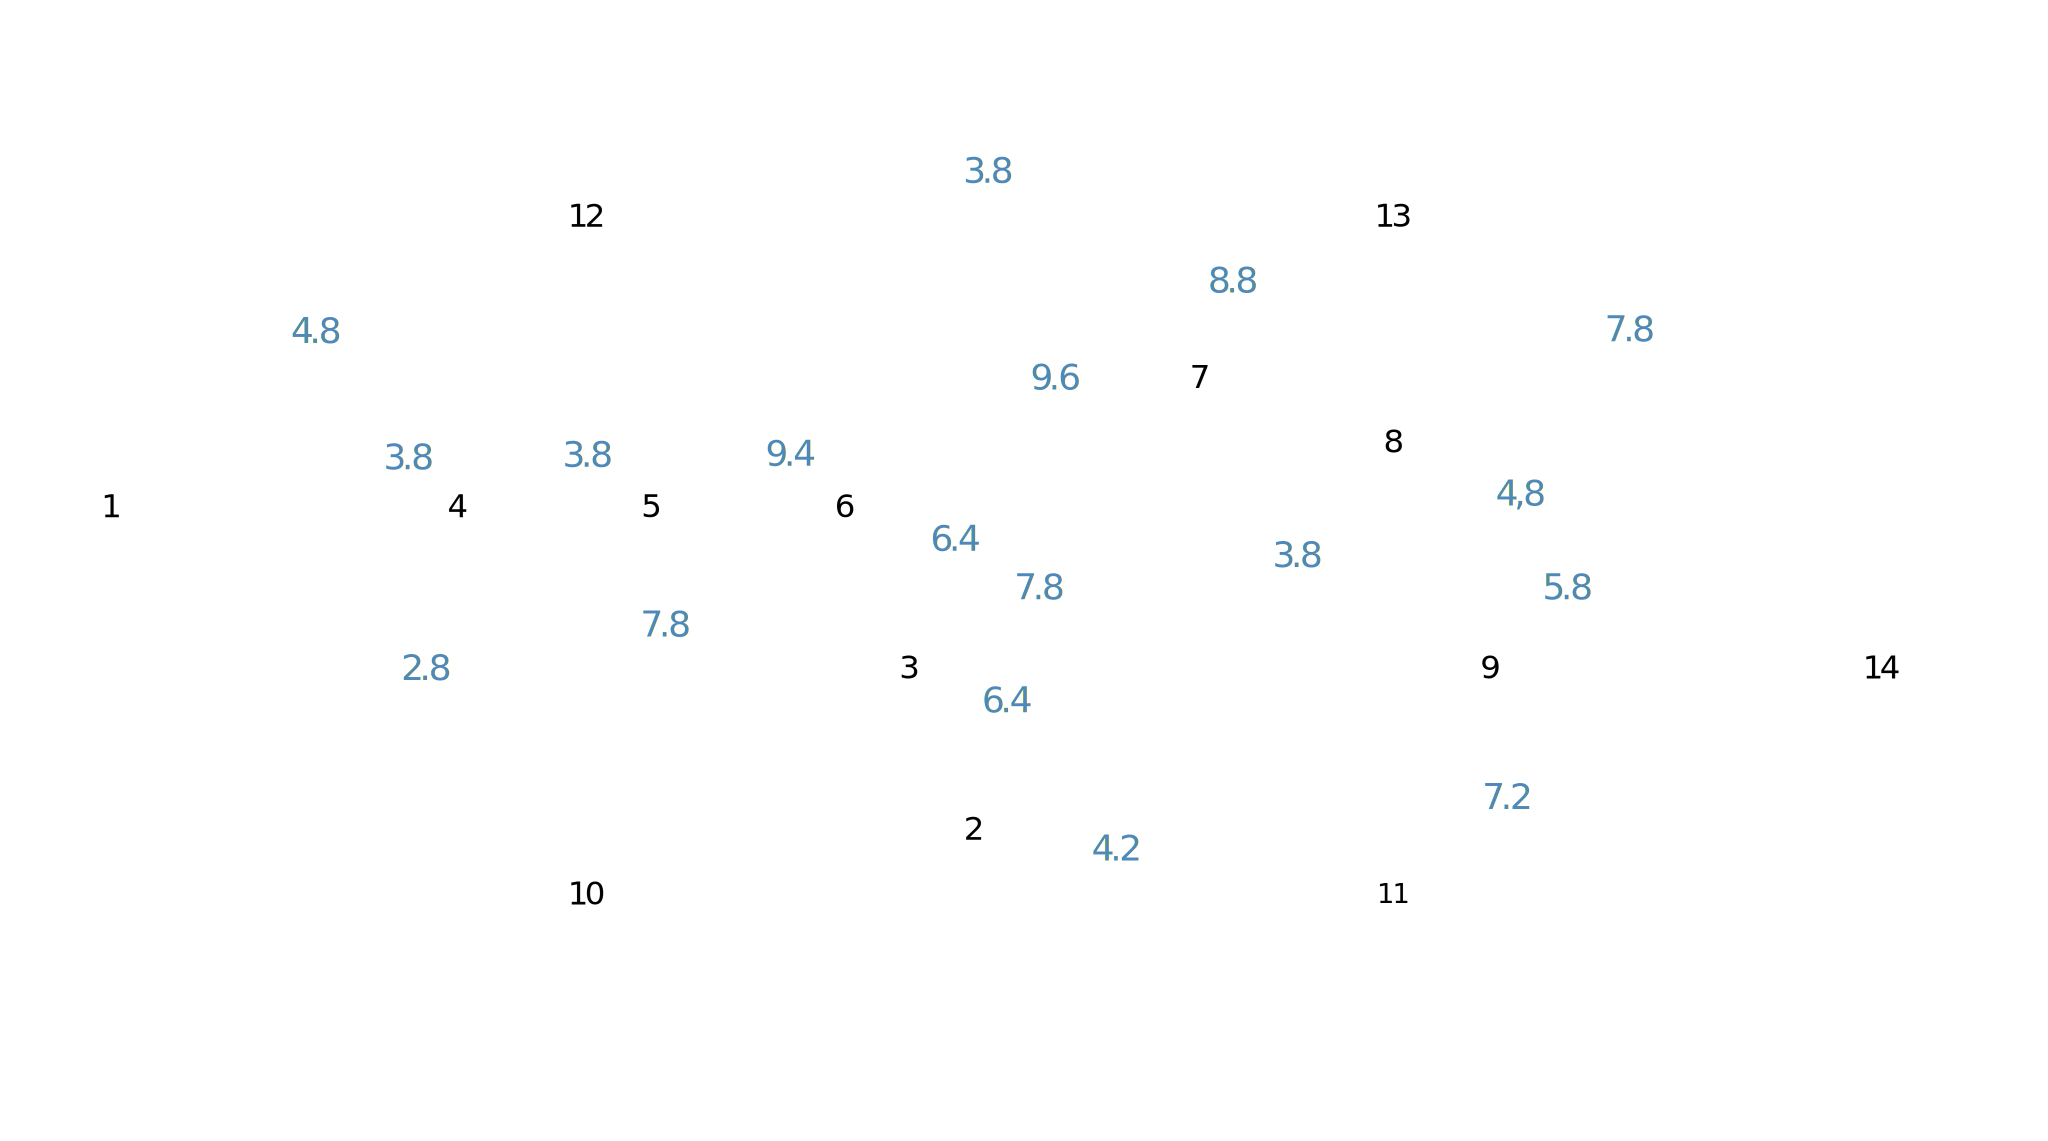
\includegraphics[bb=0 0 437 243]{Setevoy_Grafik.jpg}
\caption{Сетевой график}
\end{figure}
\\
\subsection{Анализ сетевой модели.}

{\itshape Путём} в сетевой модели называется последовательность работ, соединя\-ющая две любые работы на графике (если такая последовательность сущест\-вует).
Введём обозначения: $L_{1(i)}$ - путь, предшествующий событию $i$, $L_{2(i)}$ - путь, следующий за событием $i$.

Критический путь на сетевой модели (последовательность событий от начала проекта к концу проекта, имеющая максимальную длину):
$$
L = 1-4-5-6-3-2-7-8-9-14
$$

Длина пути $T(L) = \sum\limits_{i-j}t_{i-j}$ (где $t_{i-j}$ - длительность работы с меткой $i-j$) - сумма длительностей работ, которые выполняются при следовании по пути. Длина критического пути:
$$
T_{\mbox{кр}}(L) = 3.8+3.8+9.4+6.4+6.4+7.8+8.8+4.8+5.8 = 57 \mbox{ дней}
$$
Ранний срок наступления события: $t_{\mbox{р}(i)} = max(T(L_{1(i)}))$\\
Ранний срок начала работы: $t_{\mbox{рн}(i-j)} = max(T(L_{1(i)}))$\\
Ранний срок окончания работы: $t_{\mbox{ро}(i-j)}= t_{\mbox{р}(i)} - t_{(i-j)} = max(T(L_{1(i)})) + t_{(i-j)} $\\
Поздний срок наступления события: $t_{\mbox{п}(i)}= T_{\mbox{кр}}(L) -  max(T(L_{2(i)}))$\\
Поздний срок начала работы: $t_{\mbox{пн}(i-j)}= t_{\mbox{по}(i)} - t_{(i-j)}$\\
Поздний срок окончания работы: $t_{\mbox{по}(i-j)} = t_{\mbox{п}(j)}= T_{\mbox{кр}}(L) -  max(T(L_{2(i)}))$\\
Общий резерв времени работы: $R_{(i-j)} = t_{\mbox{по}(i-j)} - t_{\mbox{ро}(i-j)} =  t_{\mbox{п}(j)} -  t_{\mbox{р}(j)} -  t_{(i-j)}$\\
Свободный резерв времени работы: $r_{(i-j)} = t_{\mbox{р}(i-j)} - t_{\mbox{ро}(i-j)} =  t_{\mbox{р}(j)} -  t_{\mbox{р}(i)} -  t_{(i-j)}$\\
Резерв времени события: : $r_{(i)} = t_{\mbox{п}(i)} - t_{\mbox{р}(i)} $

Результат расчёта параметров для сетевой модели работы над дипломным проектом представлен в таблице:

\begin{center}
Таблица 2.3: Параметры сетевой модели
\end{center}
{
\footnotesize
\begin{longtable}[H]{|p{1.1cm}|p{0.5cm}|p{0.5cm}|p{1.1cm}|p{1.1cm}|p{1.1cm}|p{1.1cm}|p{0.9cm}|p{0.9cm}|p{0.9cm}|}
%\caption{Параметры сетевой модели \label{psm}}\\
%\caption{\label{psm}}\\
\hline
Шифр & $t_{exp}$ & $\sigma$ &  $t_{\mbox{рн}(i-j)}$ $t_{\mbox{р}(i)}$ & $t_{\mbox{ро}(i-j)}$ & $t_{\mbox{пн}(i-j)}$ & $t_{\mbox{по}(i-j)}$ $t_{\mbox{п}(j)}$ & $R_{(i-j)}$ & $r_{(i-j)}$ & $r_{(i)}$\\
\hline
1-4&3,8&0,36&0&3,8&8,8&12,6&8,8&0&8,81\\
\hline
1-12&4,8&0,36&0&4,8&49,4&54,2&49,4&0&49,4\\
\hline
1-10&2,8&0,36&0&2,8&51,6&54,4&51,6&1,4&51,6\\
\hline
2-7&7,8&0,36&29,8&37,6&38,6&46,4&8,8&0&8,8\\
\hline
3-2&6,4&0,64&23,4&23,4&32,2&38,6&15,2&6,4&15,2\\
\hline
4-5&3,8&0,36&3,8&7,6&12,6&16,4&8,8&2,7&8,8\\
\hline
5-6&9,4&0,64&7,6&17&16,4&25,8&8,8&9,6&8,8\\
\hline
5-2&7,8&0,36&15,4&15,4&30,8&38,6&23,2&14,4&23,2\\
\hline
6-3&6,4&0,64&17&23,4&25,8&32,2&8,8&0&8,8\\
\hline
6-7&9,6&0,04&26,6&26,6&36,8&46,4&19,8&11&19,8\\
\hline
7-8&8,8&0,36&37,6&46,4&46,4&55,2&8,8&0&8,8\\
\hline
7-9&3,8&0,36&37,6&51,2&56,2&60&8,8&0&8,8\\
\hline
8-9&4,8&0,36&46,4&51,2&55,2&60&8,8&0&8,8\\
\hline
9-14&5,8&0,36&51,2&57&60&65,8&8,8&0&8,8\\
\hline
10-11&4,2&0,16&2,8&7&54,4&58,6&51,6&0,2&51,6\\
\hline
11-14&7,2&0,16&7&14,2&58,6&65,8&51,6&0&51,6\\
\hline
12-13&3,8&0,36&4,8&8,6&54,2&58&49,4&0&49,4\\
\hline
13-14&7,8&0,36&8,6&16,4&58&65,8&49,4&0&49,4\\
\hline
\end{longtable}
%\end{myTableSecond}
}

Директивный срок выполнения проекта составляет 122 дня, при этом длина критического пути 57 дней – таким образом, проект будет завершён в срок и нет необходимости перестраивать сетевой график проекта. Сумма дисперсий работ, лежащих на критическом пути, составляет 4.08. Среднеквад\-ратическое отклонение для критического пути составляет $\sqrt{4.08} = 2.02$ . Доверительный интервал для срока выполнения всех работ имеет вид $[50.6-2.02,50.6+2.02 ] \sim [30.58, 52.62]$. Вероятность выполнения работы в срок составляет $P=\Phi((122-50.6)/2.02)=\Phi(35.3)\sim 1$, где $\Phi(x)$ – функция Лапласа.

\section{Расчет затрат}
\label{rz}

В разделе описаны основные затраты разработчика, влияющие на це\-ну конечного продукта: расходные материалы, аренда помещений, зара\-ботная плата и т.д.

\subsection{Материальные}

Для выполнения дипломного проекта требуется приобрести следующие материальные активы: шариковые ручки, бумагу формата А4, картридж для принтера, скрепки для степлера. Количество материалов, а так же их стоимость приведены в таблице \ref{materials}:

\begin{table}[H]
\caption{Материалы \label{materials}}
\begin{center}
\begin{tabular}{|p{3.5cm}|p{3.6cm}|p{3.6cm}|p{3.4cm}|p{3.4cm}|}
\hline
Товар & Цена (руб.) & Количество (шт.) & Сумма (руб.)\\
\hline
Ручка &40 &5 &200\\
\hline
Скрепки &2 &20 &40 \\
\hline
Файл для бумаг &3 &10 &30\\
\hline
Пачка бумаги А4(200шт) &150 &1  &150\\
\hline
Картридж &400 &4 &1600\\
\hline
\multicolumn{3}{|c|}{Итого}& 2020 \\
\hline
\end{tabular}
\end{center}
\end{table}

Таким образом, материальные затраты на написание диплома составляют $M=2020$ руб.

\subsection{Заработная плата}
\label{zp}

При работе над экономической частью дипломного проекта необходимо рассчитать заработную плату сотрудникам, задействованным в работе над дипломом.

В работе над дипломным проектом принимают участие научный руково\-дитель, студент, консультанты. Для каждого специалиста вычисляется объём заработной платы, исходя из почасовой ставки и  времени, в течение которого специалист участвует в проекте.

Расчёты приведены в таблице \ref{zp2013}, данные по заработной плате научных ру\-ководителей и консультантов соответствуют зарплатам в Московском авиа\-ционном институте за 2013 г. Оплата для студента, выполняющего дипломную работу, соответствует размеру стипендии.
\begin{table}[H]
\caption{Заработная плата \label{zp2013}}
\begin{center}
\begin{tabular}{|p{3.5cm}|p{1.8cm}|p{1.6cm}|p{2.8cm}|p{2.1cm}|p{1.8cm}|}
\hline
Специалист&Заработ\-ная плата&Коли\-чество часов &Количество часов на одного дипломника&Почасовая оплата&Заработ\-ная плата\\
\hline
Научный руководитель&40000&90&24&444&10666\\
\hline
Консультант по экономической части&40000&90&2&444&888\\
\hline
Консультант по охране труда и окружающей среды&40000&48&2&833&1666\\
\hline
Студент&3000&-&-&-&12000\\
\hline
\multicolumn{5}{|c|}{Итого}&25220\\
\hline
\end{tabular}
\end{center}
\end{table}

Итого затраты на заработную плату составят Z = 25220 руб.

\subsection{Расходы на амортизацию оборудования}

Оборудование, которое использовалось в ходе выполнения дипломной ра\-боты, подлежит амортизации. Амортизации подвергаются основные средства и нематериальные активы для переноса части их стоимости в цену произво\-димой продукции.

Основным оборудованием (средством производства) является ноутбук DE\-LL Vostro 1440 стоимостью N = 21459 руб. Расчет амортизации произведём линейным способом:
$$
A = \frac{S\cdot n \cdot t}{ 100 \cdot T}
$$

В таблице \ref{ammort} приведены расшифровка и значения переменных формулы:
\begin{table}[H]
\caption{Амортизация оборудования \label{ammort}}
\begin{center}
\begin{tabular}{|p{3.0cm}|p{3.8cm}|p{2.6cm}|}
\hline
Переменная&Описание&Значение\\
\hline
S&Стоимость оборудования&21459 руб.\\
\hline
n&Годовая норма амортизации&20 \%\\
\hline
t&Время работы оборудования&252 часа\\
\hline
T&Эффективный срок работы оборудования&1800 часов\\
\hline
\end{tabular}
\end{center}
\end{table}

Произведём расчёт согласно данным таблицы:
$$
A = \frac{21459\cdot 20 \cdot 252}{ 100 \cdot 1800} = 601 \mbox{ (руб.)}
$$

Таким образом, амортизация ноутбука за период написания диплома со\-ставит 601 руб.

\section{Социальные отчисления}

Работодателю необходимо произвести социальные отчисления с зарплаты работников в следующем размере:
\\
Взносы в ФФОМС: 5.1\%\\
Взносы в ФСС: 2.9\%\\
Взносы в Пенсионный фонд: 22\%

Таким образом, на затраты на социальные отчисления составят (с учётом фонда оплаты труда из пункта \ref{zp} «Заработная плата»)
$$
P = Z \cdot (5.1 + 2.9 + 22)\% = Z \cdot 30 = 25220 \cdot 30\% = 7566 \mbox{ (руб.)}
$$

Итого, размер социальных выплат составит $7566$ руб.

\section{Прочие расходы}

\subsection{Транспортные расходы}

Затраты на транспорт фигурируют в работе над дипломным проектом, т.к. встречи между участниками проекта происходят на территории МАИ и каждый из работников затрачивает денежные средства на то, чтобы добрать\-ся до института. Предполагается, что все участники добираются до на метро.

В таблице \ref{transport} для каждого участника учтено количество поездок (опреде\-ляется исходя из этапов работы над дипломом), а так же полные затраты на транспорт за период написания диплома:
\begin{table}[H]
\caption{Транспортные расходы \label{transport}}
\begin{center}
\begin{tabular}{|p{3.5cm}|p{2.8cm}|p{2.6cm}|p{2.8cm}|}
\hline
Специалист&Количество поездок&Стоимость 1-ой поездки&Итого\\
\hline
Научный руководитель&16&&448\\
\cline{1-2}\cline{4-4}Консультант по экономической части&2&&56\\
\cline{1-2}\cline{4-4}Консультант по охране труда и окружающей среды&2&28&56\\
\cline{1-2}\cline{4-4}Студент&20&&560\\
\hline
\multicolumn{3}{|c|}{Итого}&1120\\
\hline
\end{tabular}
\end{center}
\end{table}

Итого расходы на транспорт составляют M = 1120 руб.

\subsection{Связь}

К прочим расходам относятся так же расходы на мобильную связь. Исходя из того, что стоимость одного комплексного тарифного плана оператора со\-товой связи <<МТС>>, включающего 300 минут разговоров и неограниченное количество смс составляет 500 руб. для каждого участника разработки дип\-лома, то за 4 месяца для 4-х человек получаем
$$
B = 500 \cdot 4 \cdot 4 = 8000 \mbox{ (руб.)}
$$

Итого, расходы на связь составляют 8000 руб.

\subsection{Интернет}

Ежемесячная абонентская плата за Интернет составляет 200 руб, общая продолжительность дипломного проекта составляет 4 месяца. Таким образом, затраты на Интернет в течение периода составляет
$$
S = 200 \cdot 4 = 800
$$

Итого, расходы на Интернет составляют $S = 800$ руб.

\subsection{Электроэнергия}

Тарифы на электроэнергию в Москве составляют 4р/КВтч. Ежедневное энергопотребление работающего компьютера составляет 50 КВт за 4 часа работы. С учётом 7-ми дневной рабочей недели, получаем за 4 месяца. 
$$
E = 50 \cdot 7 \cdot 4 \cdot 4 = 11200
$$

Таким образом, окончательно получаем
$$
Y = 800 + 8000 +1120 + 11200= 21120
$$

Итого, прочие расходы составляют 21120 руб.


\section{Расчет экономической эффективности}

Для расчёта экономической эффективности нужно вычислить себесто\-имость продукта, его цену продажи, а так же экономический эффект, который ожидается от внедрения продукта

\subsection{Расчёт цены на продукт}

Чтобы рассчитать цену на продукт, необходимо вычислить его себесто\-имость. Себестоимость продукта с определяется как сумма всех затрат, вы\-численных в пункте \ref{rz} «Расчет затрат».\\
\begin{math}
SS = M + Z + A + P + Y = \\ 
= 2020 + 25220 + 601 + 7566 + 21120 = 56527 \mbox{ руб.}
\end{math}

Норма прибыли равна 5\%. НДС, который так же нужно учесть в цене, составляет 18\%. Тогда цена на продукт составит
$$
C = 56527 \cdot (100\% + 5\% + 18\%) = 63876 \mbox{ (руб.)}
$$

\section{Экономический эффект}

Экономический эффект, который принесёт внедрение доработок в систему дистанционного обучения, заключается в ликвидации недополученной при\-были за дополнительные занятия для студентов.

После внедрения системы появится возможность выделить среди группы студентов, проходящих курсы в системе дистанционного обучения, тех поль\-зователей, которые решают задачи теста с заранее имеющимися ответами.

Если студент использует  готовые ответы – он не до конца освоил нужный курс и нуждается в дополнительных занятиях. Оценим прибыль, которую институт может получить за один семестр по формуле:
$$
L = N \cdot i \cdot k \cdot V
$$

\newpage
В таблице \ref{profit} приведены расшифровка и значения переменных в формуле.
\begin{table}[H]
\caption{Экономический эффект\label{profit}}
\begin{center}
\begin{tabular}{|p{3.0cm}|p{4.1cm}|p{2.6cm}|}
\hline
Переменная&Описание&Значение\\
\hline
N&Количество студентов &430\\
\hline
i&Доля воспользовавшихся ответами&15 \%\\
\hline
k&Стоимость одного доп. занятия на курсах&540 руб.\\
\hline
V&Количество доп. занятий&4 шт\\
\hline
\end{tabular}
\end{center}
\end{table}

Таким образом, получаем:
$$
L = N \cdot i \cdot k \cdot V = 450 \cdot 15 \cdot 540 \cdot 4 =  139320 \mbox{ (руб.)}
$$

Итого, экономический эффект от модификации системы дистанционного обучения сос\-тавит 139320 руб в семестр.

\subsection{Экономическая эффективность}

Для расчёта экономической эффективности необходимо учесть расходы на внедрение системы и эксплуатацию сервиса.

Расходы на внедрение системы  вычисляются по формуле 
$$
C_{\mbox{вн}} = t_{\mbox{вн}}\cdot p,
$$
где $t_{\mbox{вн}} = 3$ часа - время, необходимое для установки системы на сервер и $p=630$ руб - почасовая ставка программиста, который занимается развёр\-тыванием системы
$$
C_{\mbox{вн}} = 3 \cdot 630 = 1890 \mbox{ (руб.)},
$$

Расходы на эксплуатацию сервиса складываются из затрат на оплату сервера, который использует система дистанционного обучения:
$$
C_{\mbox{эксп}} = t_{\mbox{эксп}}\cdot c,
$$

где $t_{\mbox{эксп}} = 6$ мес. (расчёты производим за семестр) и  $c = 1200$ руб. – помесячная оплата сервера. Тогда
$$
C_{\mbox{эксп}} = 6 \cdot 1200 = 7200 \mbox{ (руб.)}.
$$ 

Итого получаем срок окупаемости вложенных средств:
$$
T_{\mbox{ок}} = \frac{C_{\mbox{эксп}} + C_{\mbox{вн}} + C}{L} = \frac{7200+1890+63876}{139320} = 0.52 (\mbox{ семестра})
$$

Таким образом средства, вложенные в систему, будут возвращены в течение половины семестра.

\section{Вывод} 
В экономической части дипломной работы был произведён расчёт се\-бестоимости и цены продажи проекта.

Построен сетевой график выполнения дипломной работы. По графику найден критический путь и рассчитаны параметры сетевой модели для каж\-дого узла. По рассчитанным параметрам произведена оценка наиболее веро\-ятного срока выполнения проекта, а так же вычислена вероятность завер\-шения проекта в срок.

Была проведена оценка затрат на введение и эксплуатацию системы, а так же оценка прибыли, которую принесёт проект. На основании этих данных определена экономическая эффективность разработанной системы.

По результатам расчётов сделан вывод о том, что вложенные в систему средства будут возвращены инвестору в течении половины учебного семестра.